\documentclass[10pt,twocolumn,letterpaper]{article}
\usepackage[utf8]{inputenc}
\usepackage{graphicx}
\graphicspath{{./}}
\usepackage{amsmath,amssymb}
\usepackage{booktabs}
\usepackage[margin=0.75in]{geometry}
\usepackage{hyperref}
\usepackage{titlesec}
\usepackage{caption}

\titleformat{\section}{\large\bfseries}{\thesection.}{0.5em}{}
\titleformat{\subsection}{\normalsize\bfseries}{\thesubsection.}{0.5em}{}
\titlespacing*{\section}{0pt}{6pt}{3pt}
\titlespacing*{\subsection}{0pt}{4pt}{2pt}
\captionsetup{font=small,skip=2pt}
\setlength{\textfloatsep}{8pt}
\setlength{\floatsep}{6pt}

\title{RegenRL: Optimizing Electric Vehicle Braking Torque Split via Soft Actor-Critic}
\author{
Rahul Choudhary (B23EE1060), IIT Jodhpur \\
GitHub: \url{https://github.com/zerokelvinrahul/RegenRL}
}
\date{}

\begin{document}
\maketitle
\vspace{-1.5em}

\begin{abstract}
\small
Electric vehicles recover braking energy through their traction motor, but regeneration is constrained by
motor back-EMF cutoffs, battery BMS charge acceptance, and road-slope axle stability, while the driver demands consistent deceleration.
We formulate the continuous regenerative-to-friction braking split as a reinforcement learning problem and solve it with Soft Actor-Critic (SAC).
Over 20 unseen test drive cycles, 3-seed SAC outperforms a validation-tuned fixed-ratio controller and an automotive-style rule-based heuristic.
Against the rule-based controller it gains $+22.1\%$ reward (paired $p=0.0026$) with $5\%$ more recovered energy and a $52\%$ lower mean stopping-distance violation ($p=0.13$, a trend rather than a significant effect).
SAC closes $47.3\%$ of the reward gap between the rule-based controller and a greedy hardware-limit reference.
\end{abstract}

\begin{figure*}[!t]
\centering
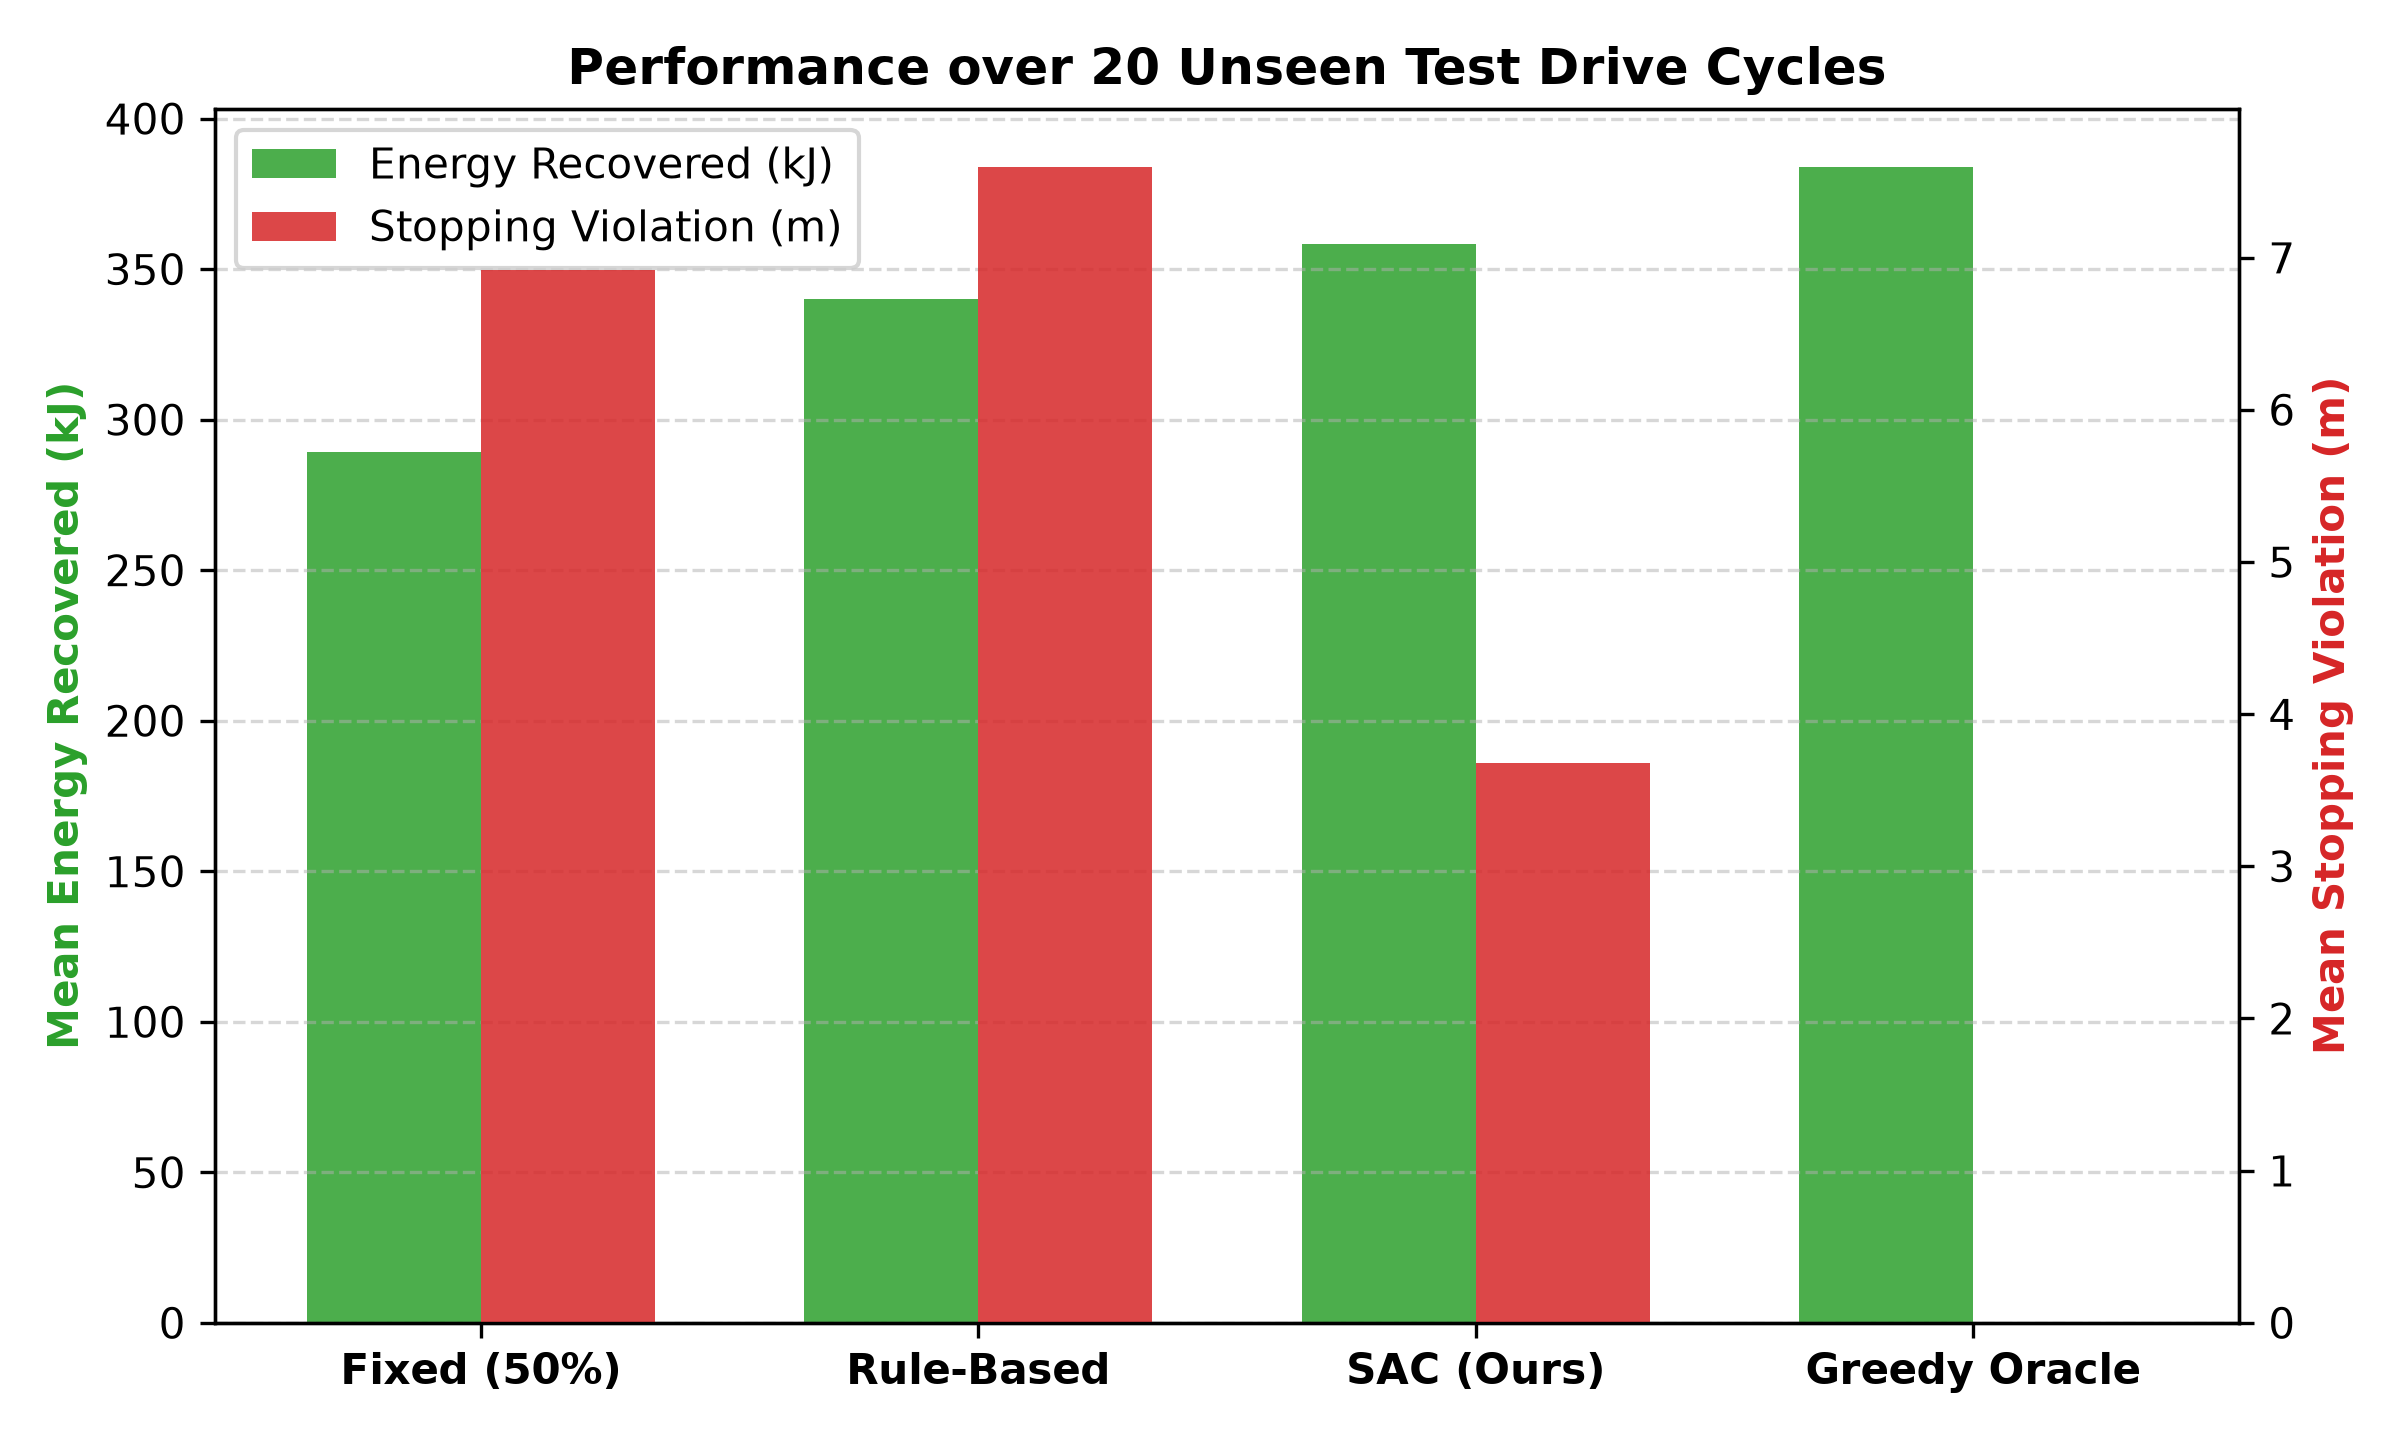
\includegraphics[width=0.325\textwidth]{bar_metrics.png}\hfill
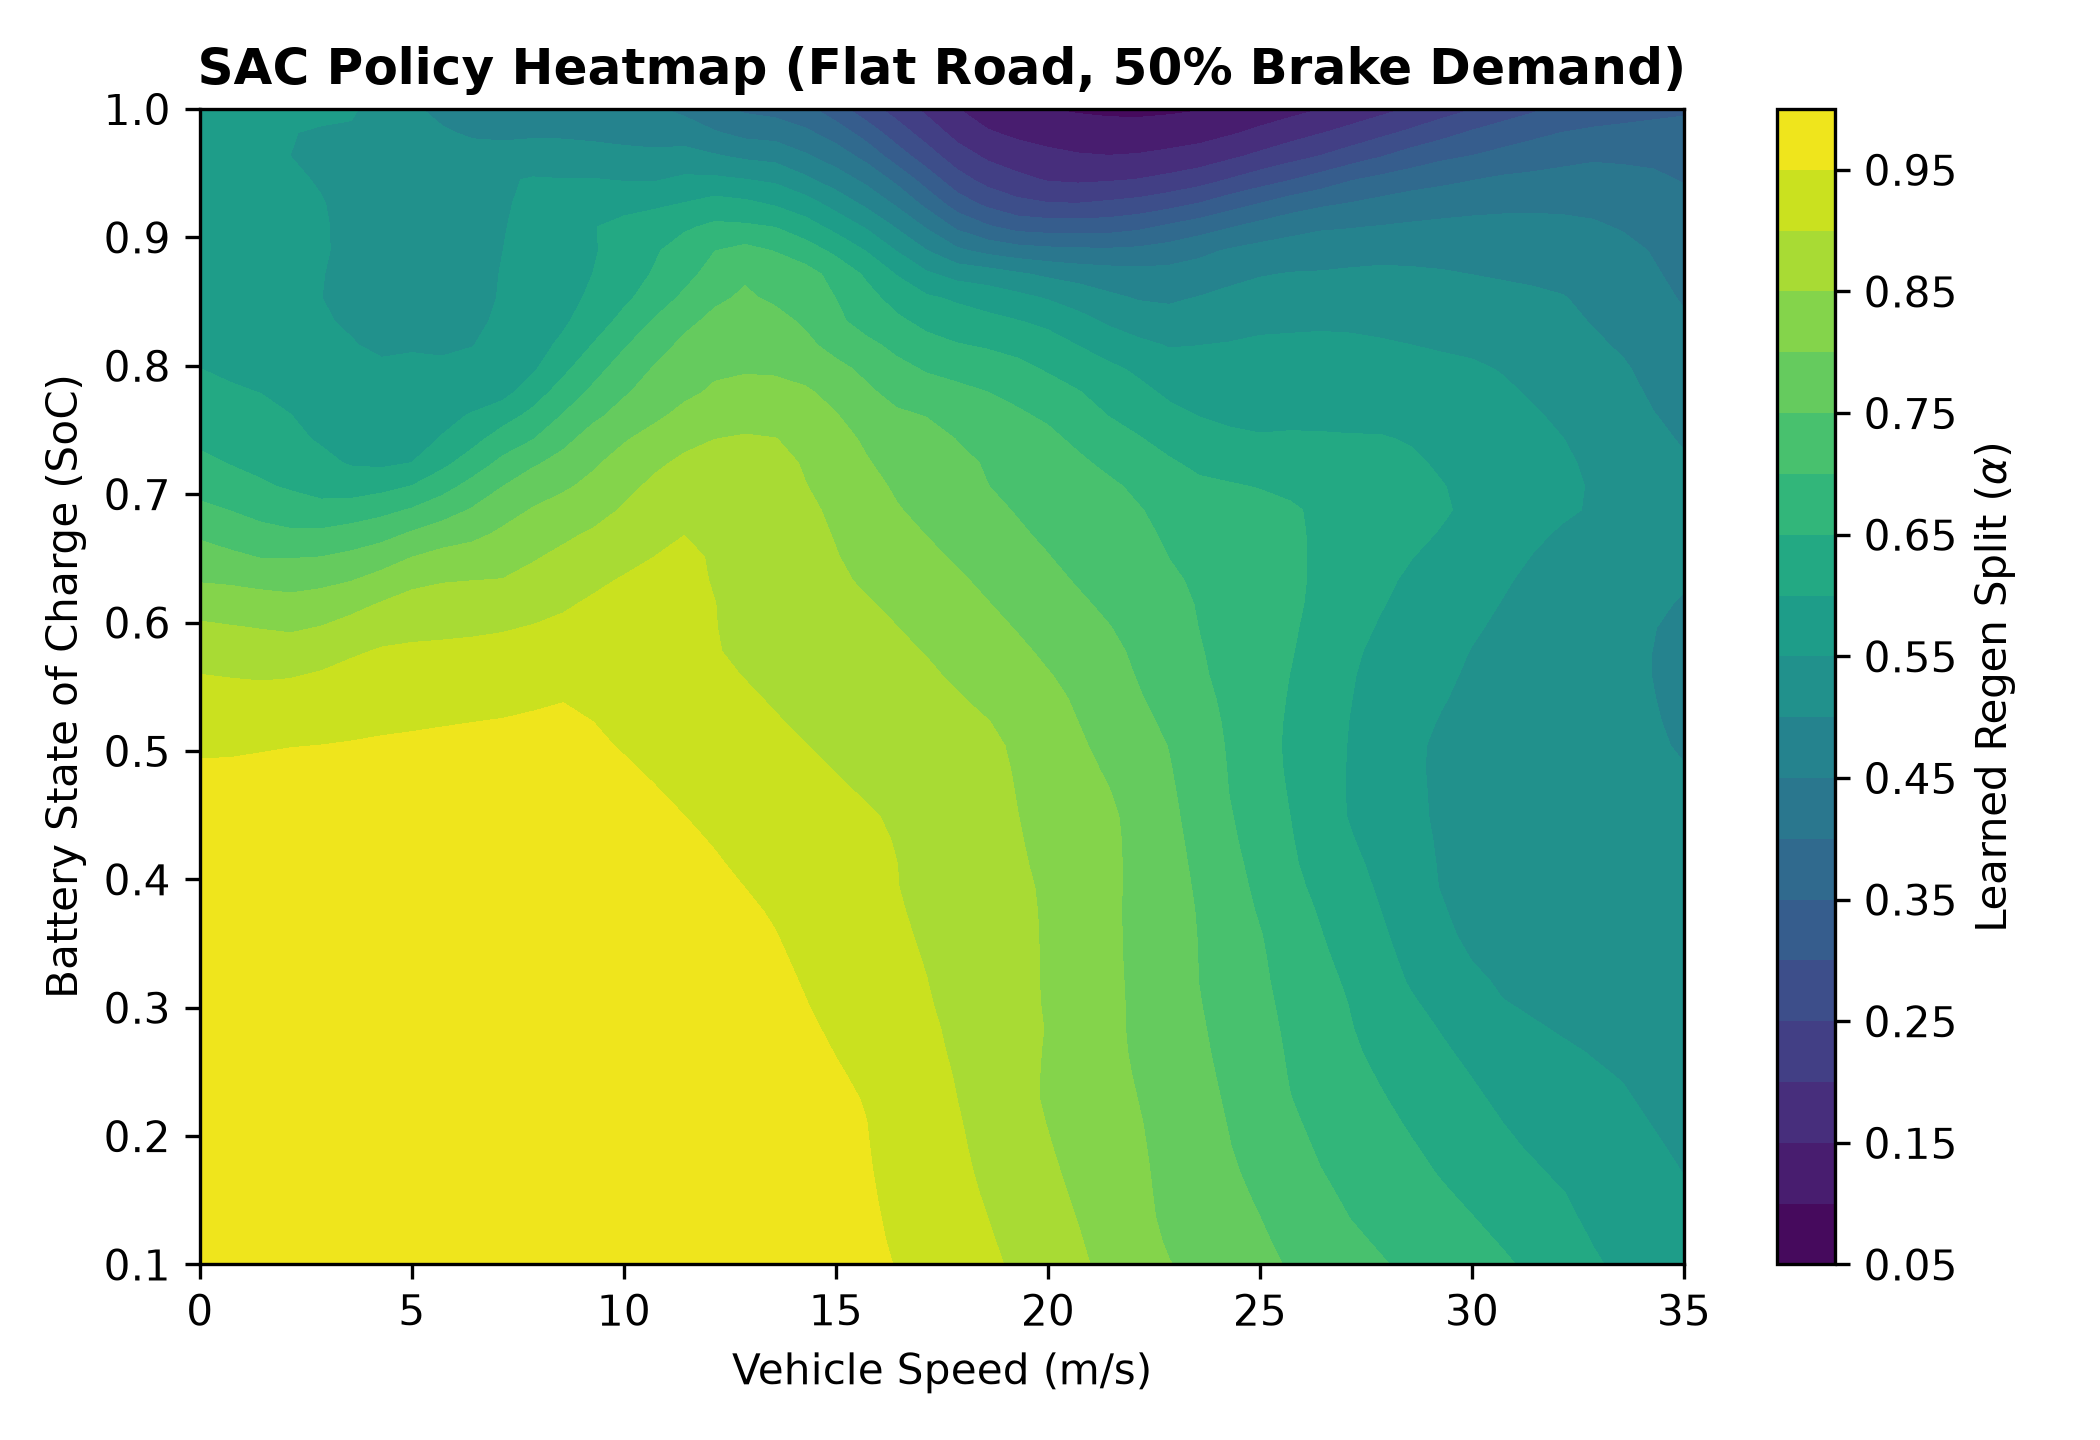
\includegraphics[width=0.325\textwidth]{heatmap.png}\hfill
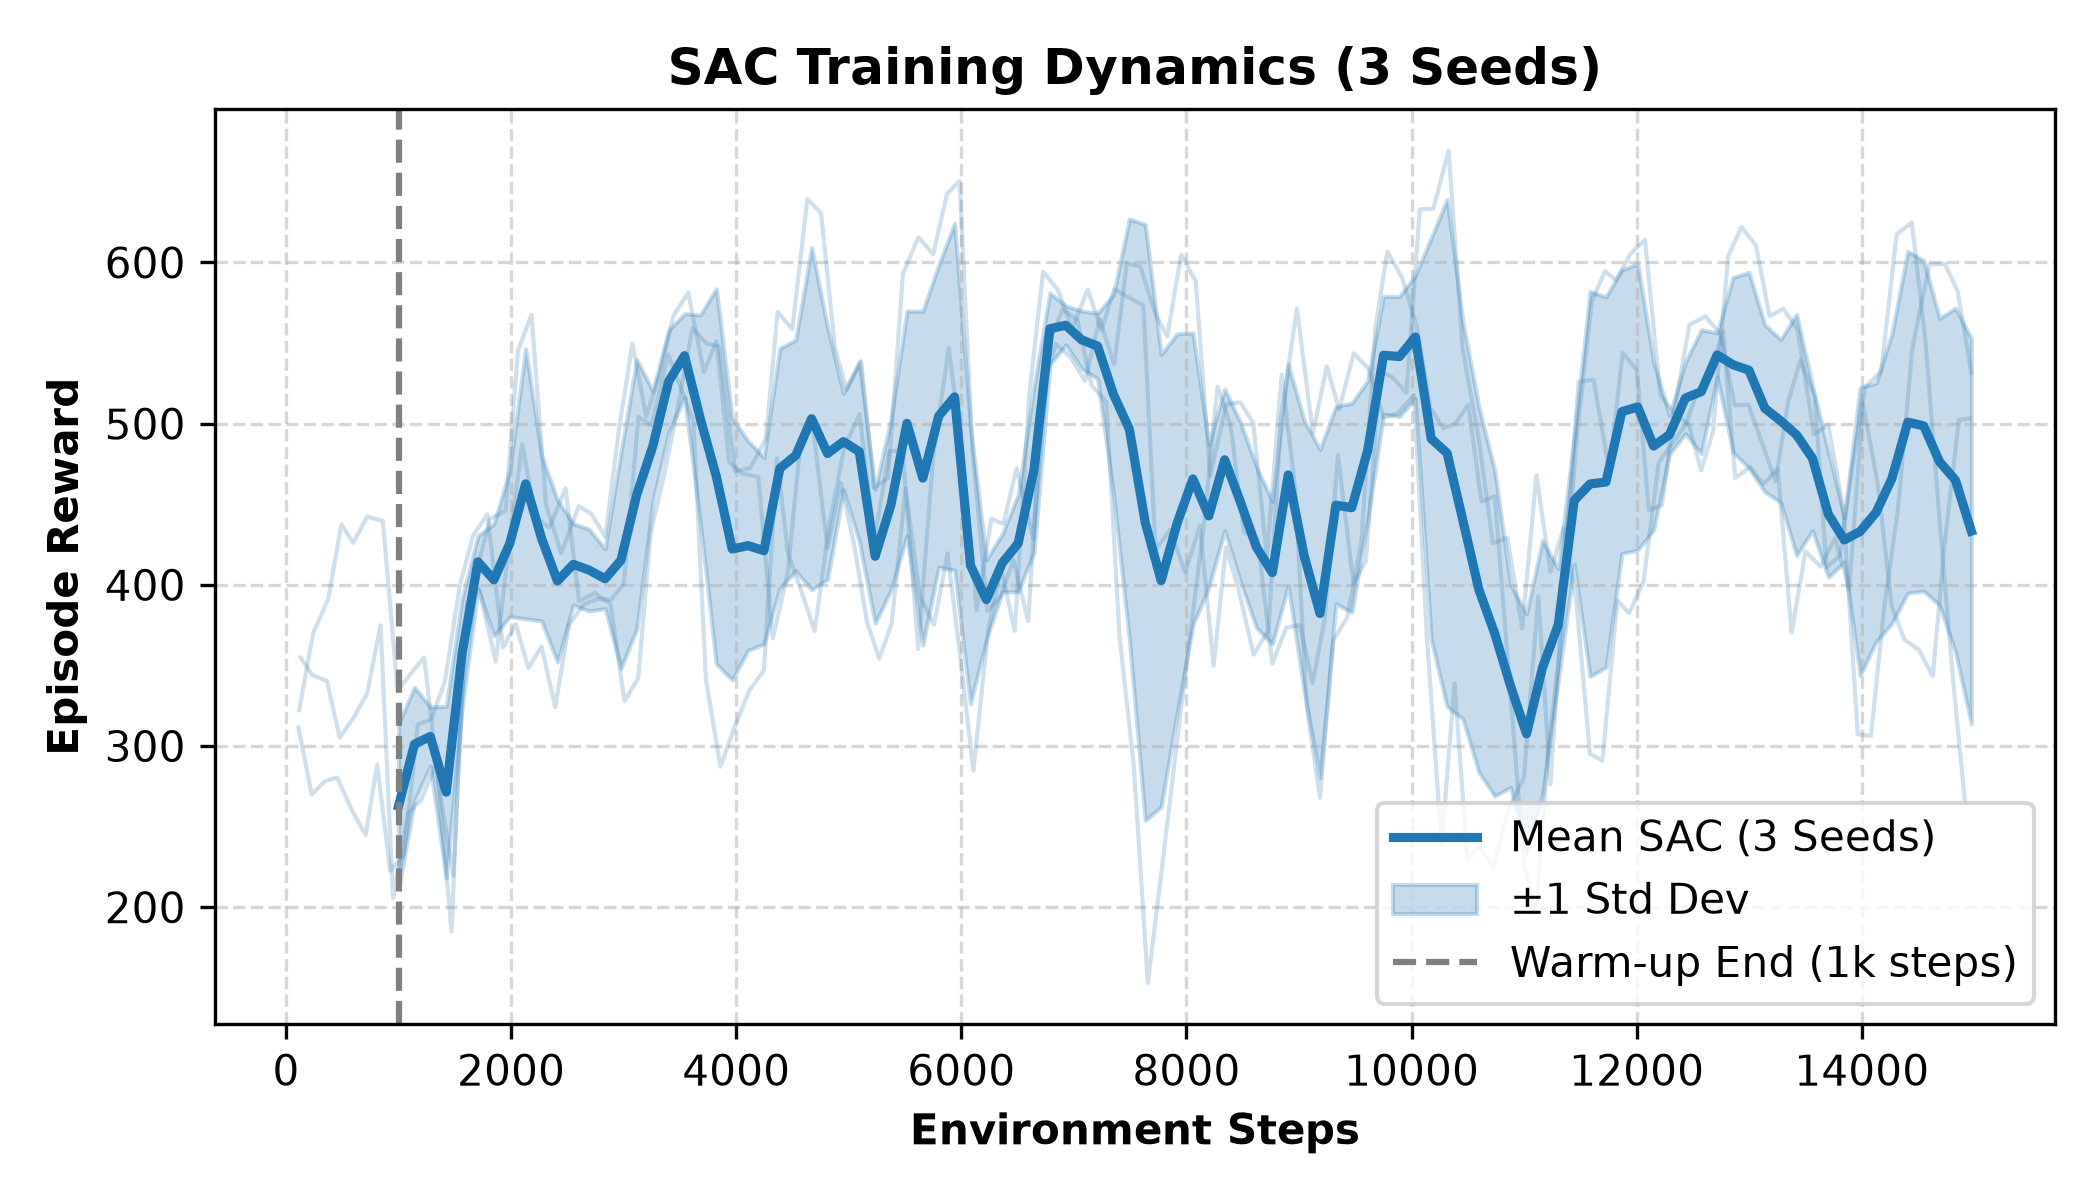
\includegraphics[width=0.325\textwidth]{training_curve.png}
\caption{Left: mean energy recovered and stopping violation over 20 test cycles (SAC averaged over 3 seeds). Middle: learned policy $\alpha(v,\mathrm{SoC})$ of the seed-42 SAC agent on flat road ($50\%$ brake demand). Right: SAC learning curves over 3 seeds with $\pm 1\sigma$ band.}\label{fig:bar}\label{fig:heat}\label{fig:train}
\end{figure*}

\section{Problem and RL Formulation}
At every 0.1\,s step the agent chooses the fraction $\alpha_t$ of the driver's torque demand $T^{dem}_t$ to be
delivered by regeneration; the rest, $(1-\alpha_t)T^{dem}_t$, goes to friction brakes. Requesting too
little regen wastes energy, while requesting more than the hardware can deliver (low speed, high SoC, high power) leaves a
torque deficit and a longer stopping distance.

\textbf{State space} $\mathcal{S}\subset\mathbb{R}^4$ (normalized):
\[
s_t=\Big[\tfrac{v_t}{35},\ \mathrm{SoC}_t,\ \tfrac{\theta_t}{10^\circ},\ \tfrac{T^{dem}_t}{2500}\Big],
\]
with speed $v\in[0,35]$\,m/s, battery state of charge, road slope $\theta\in[-10^\circ,10^\circ]$ and driver
torque demand in Nm.

\textbf{Action space} $\mathcal{A}=[0,1]$ (continuous): the regen fraction $\alpha_t$, giving the
requested regen torque $T^{req}_t=\alpha_t T^{dem}_t$.

\textbf{Reward.} A dense three-term reward balances efficiency, safety and comfort:
\begin{equation}
r_t = w_e E_t - w_v\Big(d^{viol}_t + 0.05\tfrac{T^{def}_t}{1000}\Big) - w_s(\alpha_t-\alpha_{t-1})^2,
\end{equation}
where $E_t$ is the net energy stored in the battery (kJ) after motor efficiency and $I^2R$ losses,
$d^{viol}_t = v_t\,(a^{short}_t/g)\,\Delta t$ is the stopping-distance violation caused by the deceleration
shortfall $a^{short}_t$, $T^{def}_t$ is the torque deficit (Nm), and $(w_e,w_v,w_s)=(1.5,14,0.15)$. The large $w_v$
makes safety dominant, so energy is harvested only when it does not compromise braking performance.

\section{Environment and Algorithm}
\subsection{Simulation Environment}
We built a custom Gymnasium environment (\texttt{EVBrakingEnv}) for a 1650\,kg compact EV. Each episode
consists of four braking segments (urban and highway mix) with randomized initial speed, target speed, slope,
peak torque demand (600--2400\,Nm) and initial SoC ($0.50$--$0.95$). The achieved regen torque is
$T^{act}=\min(T^{req},T^{cap})$, where $T^{cap}=\min(T^{motor},T^{batt})$ combines:
(i) a low-speed back-EMF fade (zero below 1.2\,m/s, full above 4\,m/s),
(ii) the motor constant-torque / constant-power curve (1850\,Nm, 60\,kW),
(iii) a slope-dependent axle stability factor, and
(iv) a BMS charge-power taper above 82\% SoC.
Deceleration follows from friction plus regen torque and aerodynamic, rolling and grade forces. Stored energy
accounts for a motor efficiency map (0.72--0.92) and pack $I^2R$ losses, and updates SoC.

\subsection{Algorithm: Soft Actor-Critic}
Because $\alpha_t$ is continuous, we use SAC~\cite{haarnoja2018sac,haarnoja2018apps}, an off-policy maximum-entropy
actor-critic method that maximizes $\mathbb{E}\big[\sum_t r_t+\beta\mathcal{H}(\pi(\cdot|s_t))\big]$.
The actor outputs a Gaussian squashed by $\tanh$ and rescaled to $[0,1]$. Two critics (clipped double-Q)
with soft target updates ($\tau=0.005$) reduce overestimation, and the temperature $\beta$ is tuned
automatically (target entropy $-1$). Networks have two 256-unit ReLU layers, trained with Adam
(learning rate $3\times10^{-4}$), $\gamma=0.99$, batch size 256, a 100k replay buffer, 1k random warm-up steps
and 15k environment steps per seed (seeds 42, 43, 44). The environment follows the Gymnasium API~\cite{towers2024gymnasium}.

\subsection{Baselines}
\textbf{Fixed-Ratio:} static $\alpha=0.5$, the best constant from a validation sweep over $[0.1, 1.0]$ (seeds 500--519).
\textbf{Rule-Based:} $\alpha=0.9$, linearly tapered below 8\,m/s and above 80\% SoC, mimicking automotive production logic.
\textbf{Greedy reference (oracle):} $\alpha_t = \min(1.0, T^{cap}_t / T^{dem}_t)$ using exact instantaneous hardware limits. It yields zero torque deficit and serves as an empirical upper bound, though it ignores smoothness and efficiency-map effects. All controllers are evaluated on identical test seeds.

\section{Results}
Table~\ref{tab:res} reports test metrics over 20 unseen cycles (seeds 200--219); SAC metrics are averaged over the 3 trained seeds per cycle.
Because cycle difficulty varies with speed and slope, we use paired Student's $t$-tests on per-cycle differences $\Delta = \mathrm{SAC} - \mathrm{Baseline}$.
Relative to the rule-based heuristic, SAC improves mean reward by $+22.1\%$ ($+86.78$, 95\% CI $[34.5,139.1]$, paired $t=3.472$, $p=0.0026$, win rate $80\%$) while recovering $5\%$ more energy ($358.2$ vs.\ $340.2$\,kJ). Mean stopping violation falls $52\%$ (from $7.60$\,m to $3.68$\,m), but this difference alone is not significant ($p=0.13$; SAC is lower in 11 of 20 cycles).
Relative to fixed $50\%$, SAC yields $+47.2\%$ reward ($+153.75$, $t=10.429$, $p<10^{-4}$, win rate $100\%$).
Against the greedy reference ($575.8$ reward, 0\,m violation), SAC closes $47.3\%$ of the gap between the rule-based controller and the reference, while having to learn the hardware-limit map from reward alone.
Across the three training seeds, mean test reward is $479.2 \pm 5.4$ and energy $358.2 \pm 3.0$\,kJ.

\begin{table}[t]
\centering\footnotesize\setlength{\tabcolsep}{2pt}
\caption{Test performance (mean $\pm$ std over 20 test cycles; best practical method in bold; greedy reference is an empirical upper bound).}\label{tab:res}
\resizebox{\columnwidth}{!}{%
\begin{tabular}{lccc}
\toprule
Method & Reward & Energy (kJ) & Viol. (m)\\
\midrule
Fixed (50\%) & 325.5 $\pm$ 267.2 & 289.2 $\pm$ 114.0 & 6.92 $\pm$ 7.45\\
Rule-Based & 392.4 $\pm$ 215.4 & 340.2 $\pm$ 211.6 & 7.60 $\pm$ 8.73\\
SAC (3 seeds) & \textbf{479.2} $\pm$ 292.5 & \textbf{358.2} $\pm$ 167.4 & \textbf{3.68} $\pm$ 3.02\\
Greedy ref. & 575.8 $\pm$ 269.7 & 384.0 $\pm$ 179.8 & 0.00 $\pm$ 0.00\\
\bottomrule
\end{tabular}}
\end{table}

\begin{figure}[!t]
\centering
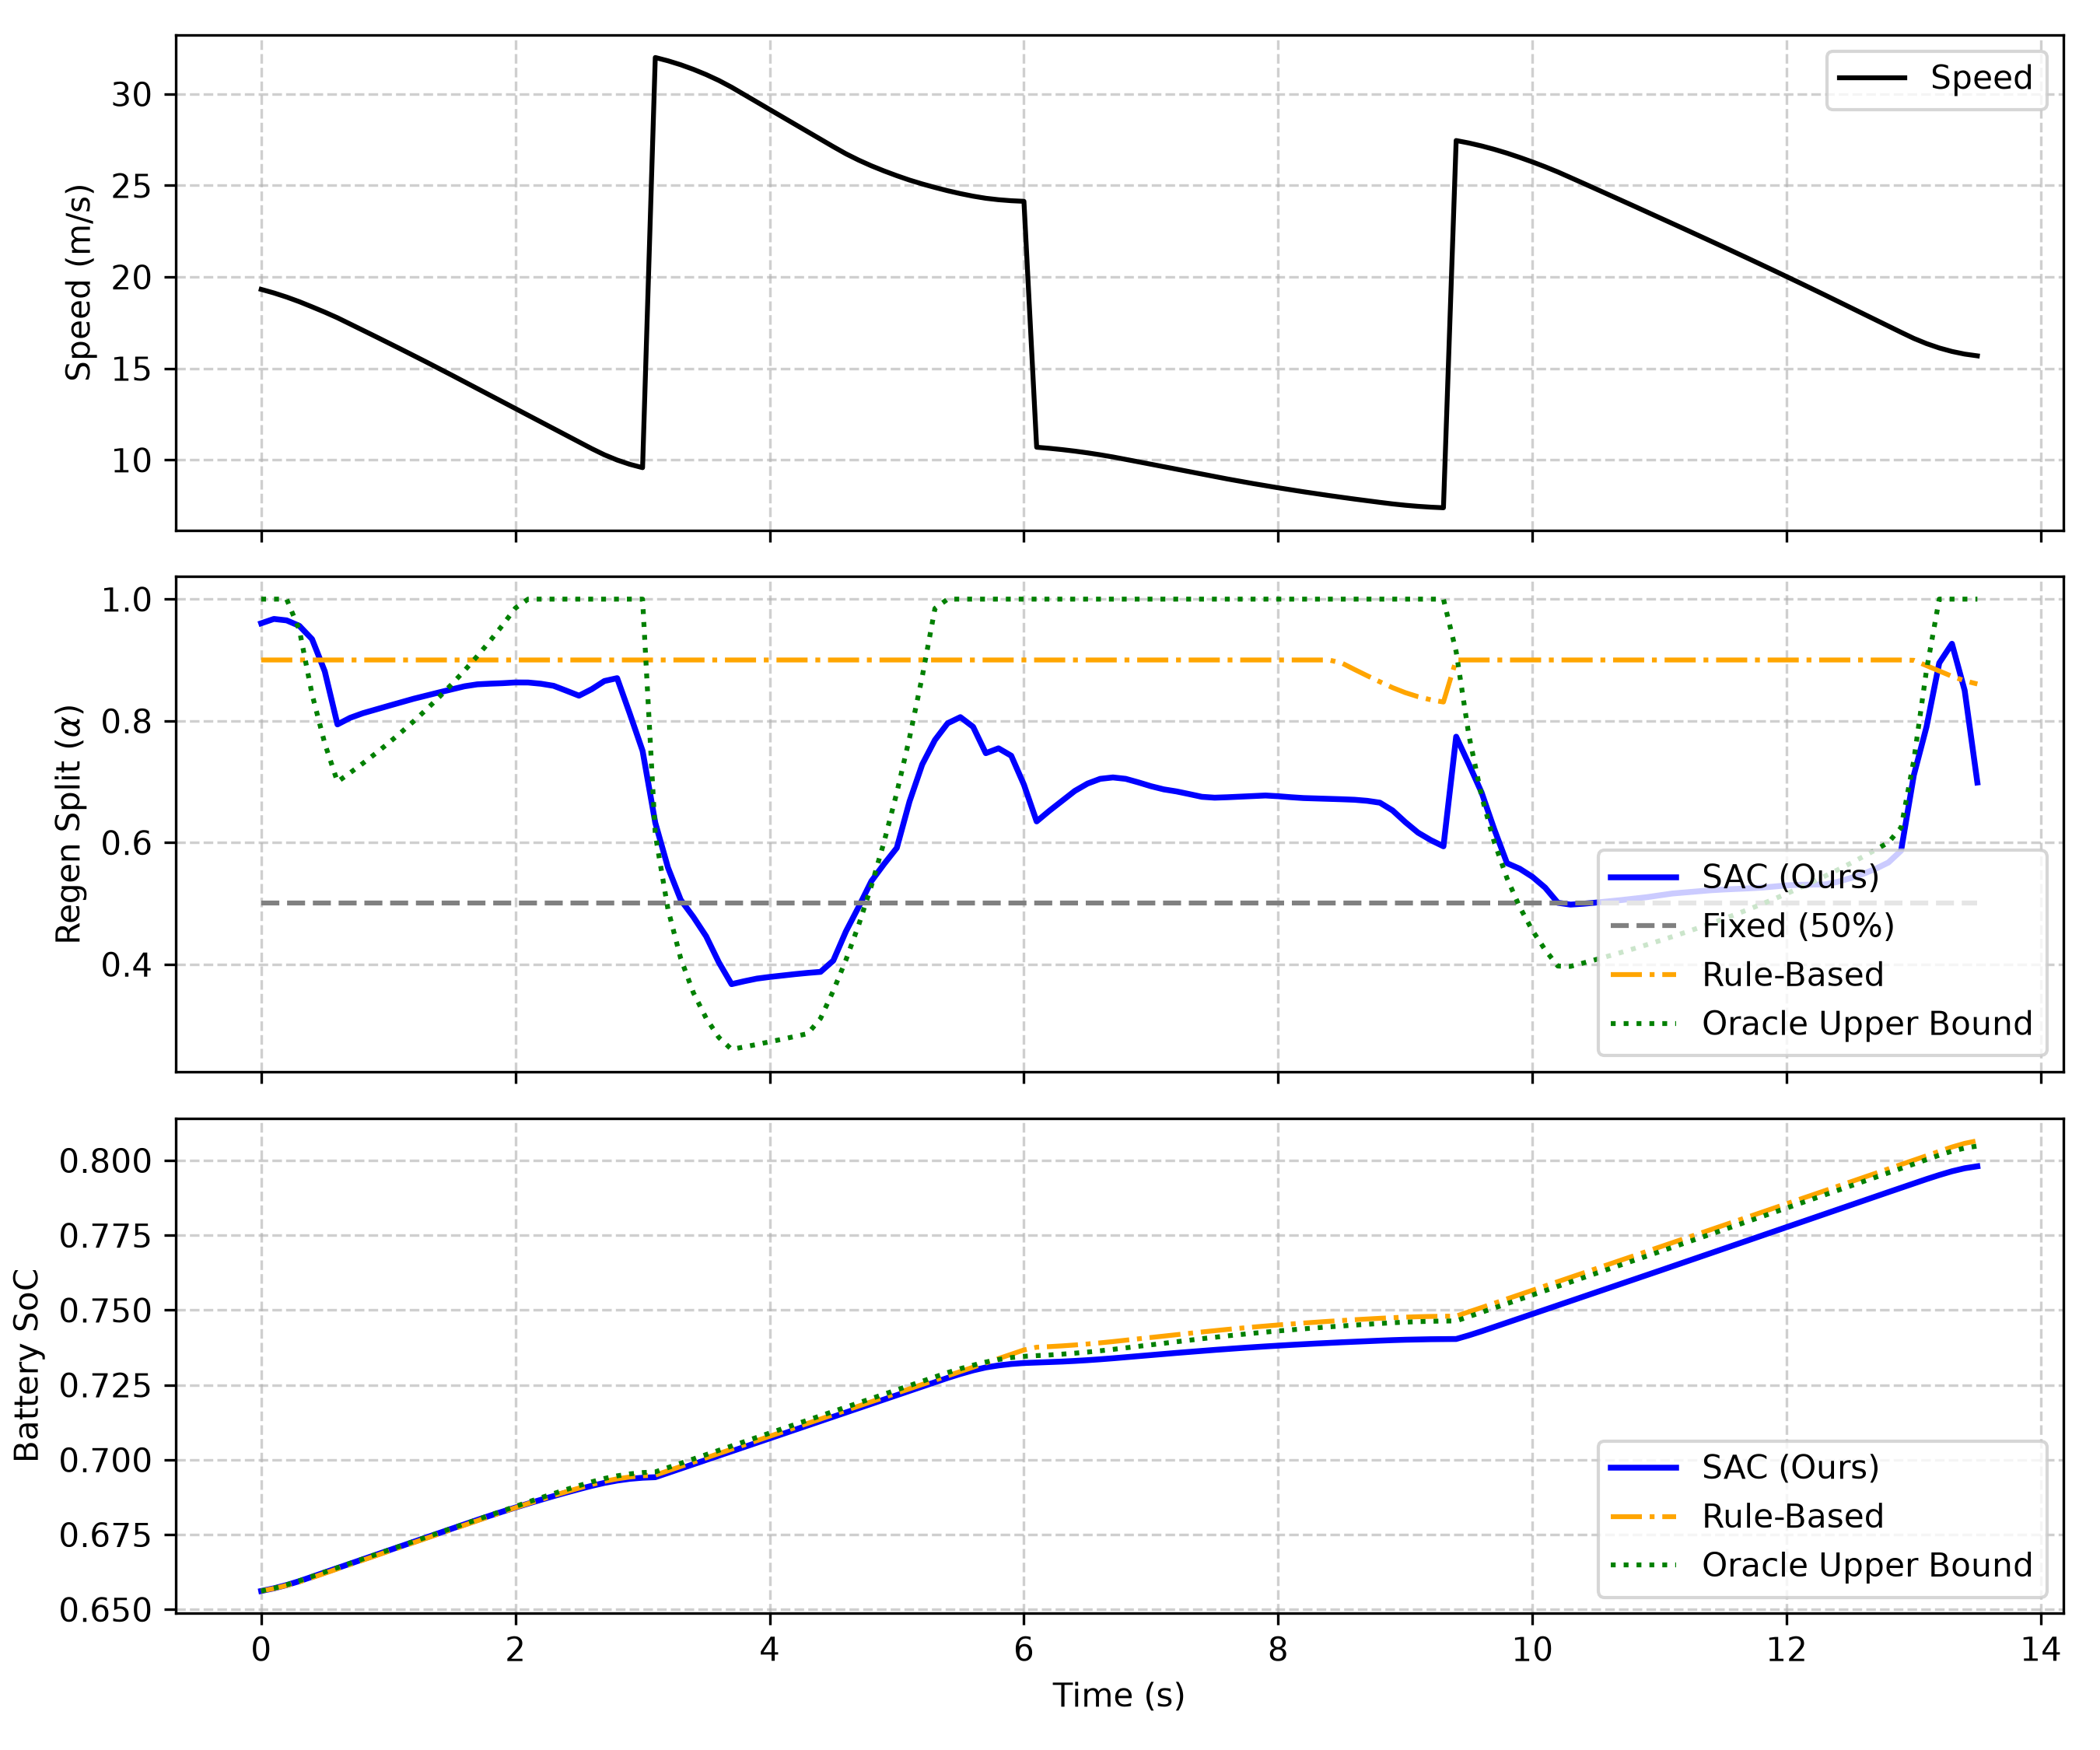
\includegraphics[width=0.95\columnwidth]{trajectory.png}
\caption{Speed, regen split $\alpha$ and SoC over one cycle (seed 101, a held-out seed outside the 200--219 test set; seed-42 SAC agent).}\label{fig:traj}
\end{figure}

\section{Discussion}
\textbf{Learned behaviour.} The trajectory (Fig.~\ref{fig:traj}) shows that SAC modulates $\alpha$ dynamically instead of holding a constant split: its $\alpha$ varies between roughly $0.4$ and $0.9$ and qualitatively follows the greedy reference, dipping where the reference dips, whereas the fixed controller stays at $0.5$ and the rule-based heuristic stays near $0.9$ throughout. Requesting $0.9$ even when the hardware cap is lower leads to torque shortfalls and stopping violations. The policy heatmap (Fig.~\ref{fig:heat}) shows $\alpha$ varying smoothly with speed and SoC, with the SoC dependence reflecting the BMS taper above 82\%.

\textbf{Training.} Reward improves quickly after the 1k-step warm-up and then fluctuates, since episodes differ in difficulty (Fig.~\ref{fig:train}); the three seeds reach similar test performance ($479.2 \pm 5.4$ reward).

\textbf{Limitations.} Variance across cycles reflects profile difficulty, which the paired tests isolate. The violation reduction versus rule-based is not statistically significant at the 5\% level. Current simplifications include independent braking maneuvers (speed resets at segment boundaries), a single-axle lumped driveline, and a 1\,kWh effective buffer window. Future work includes front/rear brake-by-wire distribution, cell thermal modeling, and continuous traffic driving schedules.

\begin{thebibliography}{9}\small
\bibitem{haarnoja2018sac} T.~Haarnoja, A.~Zhou, P.~Abbeel, S.~Levine. Soft Actor-Critic: Off-Policy Maximum Entropy Deep Reinforcement Learning with a Stochastic Actor. \emph{ICML}, 2018.
\bibitem{haarnoja2018apps} T.~Haarnoja et al. Soft Actor-Critic Algorithms and Applications. \emph{arXiv:1812.05905}, 2018.
\bibitem{towers2024gymnasium} M.~Towers et al. Gymnasium: A Standard Interface for Reinforcement Learning Environments. \emph{arXiv:2407.17032}, 2024.
\end{thebibliography}

\end{document}